% Graphic for TeX using PGF
% Title: D:\User\Documents\Individual\Coursewares\Electronics\DigitalAndAnalog\0450\src\23.dia
% Creator: Dia v0.97.2
% CreationDate: Sun Apr 14 01:36:06 2019
% For: Wu Zhenyu
% \usepackage{tikz}
% The following commands are not supported in PSTricks at present
% We define them conditionally, so when they are implemented,
% this pgf file will use them.
\ifx\du\undefined
	\newlength{\du}
\fi
\setlength{\du}{10\unitlength}
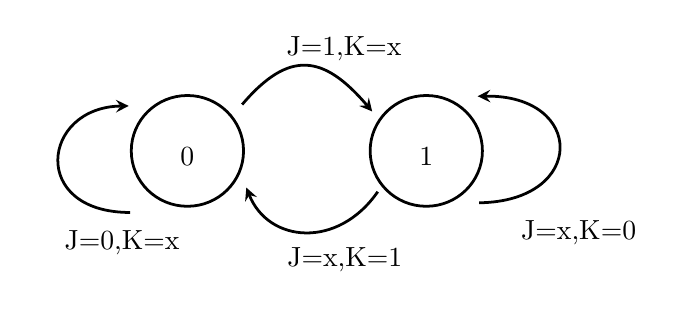
\begin{tikzpicture}
	\pgftransformxscale{1.000000}
	\pgftransformyscale{-1.000000}
	\definecolor{dialinecolor}{rgb}{0.000000, 0.000000, 0.000000}
	\pgfsetstrokecolor{dialinecolor}
	\definecolor{dialinecolor}{rgb}{1.000000, 1.000000, 1.000000}
	\pgfsetfillcolor{dialinecolor}
	\definecolor{dialinecolor}{rgb}{1.000000, 1.000000, 1.000000}
	\pgfsetfillcolor{dialinecolor}
	\pgfpathellipse{\pgfpoint{22.771664\du}{15.674982\du}}{\pgfpoint{2.028364\du}{0\du}}{\pgfpoint{0\du}{2.001682\du}}
	\pgfusepath{fill}
	\pgfsetlinewidth{0.100000\du}
	\pgfsetdash{}{0pt}
	\pgfsetdash{}{0pt}
	\pgfsetmiterjoin
	\definecolor{dialinecolor}{rgb}{0.000000, 0.000000, 0.000000}
	\pgfsetstrokecolor{dialinecolor}
	\pgfpathellipse{\pgfpoint{22.771664\du}{15.674982\du}}{\pgfpoint{2.028364\du}{0\du}}{\pgfpoint{0\du}{2.001682\du}}
	\pgfusepath{stroke}
	% setfont left to latex
	\definecolor{dialinecolor}{rgb}{0.000000, 0.000000, 0.000000}
	\pgfsetstrokecolor{dialinecolor}
	\node at (22.771664\du,15.869982\du){0};
	\definecolor{dialinecolor}{rgb}{1.000000, 1.000000, 1.000000}
	\pgfsetfillcolor{dialinecolor}
	\pgfpathellipse{\pgfpoint{31.403364\du}{15.674982\du}}{\pgfpoint{2.028364\du}{0\du}}{\pgfpoint{0\du}{2.001682\du}}
	\pgfusepath{fill}
	\pgfsetlinewidth{0.100000\du}
	\pgfsetdash{}{0pt}
	\pgfsetdash{}{0pt}
	\pgfsetmiterjoin
	\definecolor{dialinecolor}{rgb}{0.000000, 0.000000, 0.000000}
	\pgfsetstrokecolor{dialinecolor}
	\pgfpathellipse{\pgfpoint{31.403364\du}{15.674982\du}}{\pgfpoint{2.028364\du}{0\du}}{\pgfpoint{0\du}{2.001682\du}}
	\pgfusepath{stroke}
	% setfont left to latex
	\definecolor{dialinecolor}{rgb}{0.000000, 0.000000, 0.000000}
	\pgfsetstrokecolor{dialinecolor}
	\node at (31.403364\du,15.869982\du){1};
	\pgfsetlinewidth{0.100000\du}
	\pgfsetdash{}{0pt}
	\pgfsetdash{}{0pt}
	\pgfsetmiterjoin
	\pgfsetbuttcap
	{
		\definecolor{dialinecolor}{rgb}{0.000000, 0.000000, 0.000000}
		\pgfsetfillcolor{dialinecolor}
		% was here!!!
		\pgfsetarrowsend{stealth}
		\definecolor{dialinecolor}{rgb}{0.000000, 0.000000, 0.000000}
		\pgfsetstrokecolor{dialinecolor}
		\pgfpathmoveto{\pgfpoint{24.750000\du}{14.000000\du}}
		\pgfpathcurveto{\pgfpoint{26.450000\du}{12.000000\du}}{\pgfpoint{27.700000\du}{12.200000\du}}{\pgfpoint{29.450000\du}{14.250000\du}}
		\pgfusepath{stroke}
	}
	\pgfsetlinewidth{0.100000\du}
	\pgfsetdash{}{0pt}
	\pgfsetdash{}{0pt}
	\pgfsetmiterjoin
	\pgfsetbuttcap
	{
		\definecolor{dialinecolor}{rgb}{0.000000, 0.000000, 0.000000}
		\pgfsetfillcolor{dialinecolor}
		% was here!!!
		\pgfsetarrowsend{stealth}
		\definecolor{dialinecolor}{rgb}{0.000000, 0.000000, 0.000000}
		\pgfsetstrokecolor{dialinecolor}
		\pgfpathmoveto{\pgfpoint{29.650000\du}{17.150000\du}}
		\pgfpathcurveto{\pgfpoint{28.206900\du}{19.234000\du}}{\pgfpoint{25.700000\du}{19.000000\du}}{\pgfpoint{24.900000\du}{17.000000\du}}
		\pgfusepath{stroke}
	}
	\pgfsetlinewidth{0.100000\du}
	\pgfsetdash{}{0pt}
	\pgfsetdash{}{0pt}
	\pgfsetmiterjoin
	\pgfsetbuttcap
	{
		\definecolor{dialinecolor}{rgb}{0.000000, 0.000000, 0.000000}
		\pgfsetfillcolor{dialinecolor}
		% was here!!!
		\pgfsetarrowsend{stealth}
		\definecolor{dialinecolor}{rgb}{0.000000, 0.000000, 0.000000}
		\pgfsetstrokecolor{dialinecolor}
		\pgfpathmoveto{\pgfpoint{20.700000\du}{17.900000\du}}
		\pgfpathcurveto{\pgfpoint{17.050000\du}{17.900000\du}}{\pgfpoint{17.500000\du}{14.100000\du}}{\pgfpoint{20.650000\du}{14.050000\du}}
		\pgfusepath{stroke}
	}
	\pgfsetlinewidth{0.100000\du}
	\pgfsetdash{}{0pt}
	\pgfsetdash{}{0pt}
	\pgfsetmiterjoin
	\pgfsetbuttcap
	{
		\definecolor{dialinecolor}{rgb}{0.000000, 0.000000, 0.000000}
		\pgfsetfillcolor{dialinecolor}
		% was here!!!
		\pgfsetarrowsend{stealth}
		\definecolor{dialinecolor}{rgb}{0.000000, 0.000000, 0.000000}
		\pgfsetstrokecolor{dialinecolor}
		\pgfpathmoveto{\pgfpoint{33.311000\du}{17.550300\du}}
		\pgfpathcurveto{\pgfpoint{37.200000\du}{17.500000\du}}{\pgfpoint{37.150000\du}{13.650000\du}}{\pgfpoint{33.261000\du}{13.700300\du}}
		\pgfusepath{stroke}
	}
	% setfont left to latex
	\definecolor{dialinecolor}{rgb}{0.000000, 0.000000, 0.000000}
	\pgfsetstrokecolor{dialinecolor}
	\node[anchor=west] at (17.950000\du,19.000000\du){J=0,K=x};
	% setfont left to latex
	\definecolor{dialinecolor}{rgb}{0.000000, 0.000000, 0.000000}
	\pgfsetstrokecolor{dialinecolor}
	\node[anchor=west] at (26.000000\du,19.600000\du){J=x,K=1};
	% setfont left to latex
	\definecolor{dialinecolor}{rgb}{0.000000, 0.000000, 0.000000}
	\pgfsetstrokecolor{dialinecolor}
	\node[anchor=west] at (25.975000\du,11.995000\du){J=1,K=x};
	% setfont left to latex
	\definecolor{dialinecolor}{rgb}{0.000000, 0.000000, 0.000000}
	\pgfsetstrokecolor{dialinecolor}
	\node[anchor=west] at (34.450000\du,18.645000\du){J=x,K=0};
\end{tikzpicture}
